\section{Oefeningen}
\begin{oef}
Zijn de volgende verzamelingen goed gedefinieerd? Motiveer je antwoord.
\begin{enumerate}
\item De verzameling van de letters van het alfabet
\item De verzameling van grote mensen
\item De verzameling van re\"ele getallen waarvoor geldt $2x-9=16$
\item De verzameling van gehele getallen waarvoor geldt $2x-9=16$
\item De verzameling van goede voetballers
\end{enumerate}
\begin{opl}
\begin{enumerate}
\item Niet goed gedefinieerd: welk alfabet wordt er bedoeld? Zijn de hoofdletters ook element van de verzameling? Moet zijn: $\{\text{a},\text{b},\dots,\text{z},\text{A},\text{B},\dots,\text{Z}\}$
\item Niet goed gedefinieerd: wat is \emph{groot}? Moet zijn: verzameling van mensen groter dan \SI{1.80}{\meter}
\item Goed gedefinieerd
\item Goed gedefinieerd
\item Niet goed gedefinieerd: wat is \emph{goed}?
\end{enumerate}
\end{opl}
\end{oef}



\begin{oef}
Gegeven de verzameling $A=\{2,4,6,8,10\}$ en $B=\{1,3,6,7,8\}$. Welke uitspraken zijn waar? 
\begin{enumerate}
\item $2\in A$
\item $11\in B$
\item $4 \not \in B$
\item $\{2\}\in A$
\item $A\in \nat$
\item $A=\{x\mid x\in \nat \mathrm{~en~}x\mathrm{~is~even}\}$
\end{enumerate}
\begin{opl}
\begin{enumerate}
\item waar
\item niet waar
\item waar
\item niet waar: $\{2\}\subset A$ of $2\in A$
\item niet waar: $A\subset \nat$
\item niet waar: bijvoorbeeld $12\not \in A$. Zou wel waar zijn: $A=\{x\mid x\in \nat \mathrm{~en~}x\text{~is~even en }x\leqslant 10\}$
\end{enumerate}
\end{opl}
\end{oef}




\begin{oef}
Gegeven $A=\{4,\sqrt{2}, \frac{2}{3}, -2.5, -5,33,\sqrt{9},\pi \}$. Noteer volgende deelverzamelingen van $A$ door middel van opsomming:
\begin{enumerate}
\item De  getallen van $A$ die behoren tot $\nat$
\item De  getallen van $A$ die behoren tot $\integers$
\item De rationale getallen van $A$
\item De re\"ele getallen van $A$ die niet rationaal zijn
\end{enumerate}
\begin{opl}
\begin{enumerate}
\item $\{ 4,33,\sqrt{9}\}$
\item $\{ 4,33,\sqrt{9},-5\}$
\item $\{ 4,33,\sqrt{9},-5,\frac 23,-2.5\}$
\item $\{\sqrt{2},\pi\}$
\end{enumerate}
\end{opl}
\end{oef}



\begin{oef}
Waar of fout?
\begin{enumerate}
\item $\emptyset=\{0\}$
\item $x\subset \{x\}$
\item $\emptyset=\{\emptyset\}$
\item $\emptyset\in \{\emptyset\}$
\end{enumerate}
\begin{opl}
\begin{enumerate}
\item niet waar: $\emptyset=\{ \}$ of  $0\in \{0\}$ of $\emptyset\subset\{0\}$
\item niet waar: $x\in \{x\}$ of $\{x\}\subset \{x\}$
\item niet waar: $\emptyset\in\{\emptyset\}$ of $\emptyset\subset\{\emptyset\}$
\item waar
\end{enumerate}
\end{opl}
\end{oef}




\begin{oef}
\label{oef:venndiagramoef}
Bekijk figuur~\ref{fig:venndiagramoef}. De getallen 1,\dots,8 duiden een deelverzameling aan van $U$. Vul  tabel~\ref{tab:venndiagram} aan. Als voorbeeld vulden we reeds de eerste lijn in.
\begin{figure}[htbp]
\centering
% oefening venn
\begin{tikzpicture}[thick]
\draw (-4,-2.7) rectangle (4,3.5) node [above] {$U$};
\draw \firstellipse node at (35:3.7cm) {$A$};
\draw \secondellipse node at (145:3.7cm) {$B$};
\draw \thirdellipse node at (270:2.3cm) {$C$};
\node at (0,3) {1};
\node at (1.8,1.3) {2};
\node at (0,1.5) {3};
\node at (-1.8,1.3) {4};
\node at (1,0) {5};
\node at (0,0.4) {6};
\node at (-1,0) {7};
\node at (0,-1) {8};
\end{tikzpicture}
\caption{8 gebieden in een Venndiagram}
\label{fig:venndiagramoef}
\end{figure}
\begin{table}[h!tbp]
\centering
\caption{Tabel bij figuur~\ref{fig:venndiagramoef}}
\begin{tabular}{ccccc}
\toprule
$\subset A$? & $\subset B$? & $\subset C$? & Gebied & in symbolen \\ 
\midrule
N & N & N & 1  & $(A \union B \union C)^c$ \\ 
N & N & J &  &   \\ 
N & J & N &   &   \\ 
N & J & J &   &   \\ 
J & N & N &   &   \\ 
J & N & J &   &   \\ 
J & J & N &   &   \\ 
J & J & J &   &   \\ 
\bottomrule
\end{tabular} 
\label{tab:venndiagram}
\end{table}

\begin{opl}
$\qquad$ \\
\begin{table}[h!tbp]
\centering
\caption{Oplossing van oefening~\ref{oef:venndiagramoef}}
\begin{tabular}{ccccc}
\toprule
$\subset A$? & $\subset B$? & $\subset C$? & Gebied & in symbolen \\ 
\midrule
N & N & N & 1  & $(A\union B \union C)^c$ \\ 
N & N & J & 8 & $C-(A\union B)$  \\ 
N & J & N &  4 & $B-(A\union C)$  \\ 
N & J & J &7   &$(B\intersect C)-A$   \\ 
J & N & N &  2 & $A-(B\union C)$  \\ 
J & N & J & 5  & $(A\intersect C)-B$  \\ 
J & J & N & 3  & $(A\intersect B)-C$  \\ 
J & J & J & 6  & $A\intersect B\intersect C$  \\ 
\bottomrule
\end{tabular} 
\label{tab:venndiagram2}
\end{table}

\end{opl}
\end{oef}




\begin{oef}
\label{oef:oefvenn}
Gegeven $U = \{1,2,3,4,5,6,7,8\}$, $P = \{3,6\}$,  $Q =\{1,3,4,5,6,8\}$ en $R = \{3,4,8\}$.
Teken  venndiagrammen voor deze verzamelingen en plaats de elementen waar ze horen. 
\begin{opl}
Het Venndiagram van figuur \ref{fig:UPQ} op pagina \pageref{fig:UPQ} toont de oplossing.
\begin{figure}[htbp]
\centering
    \begin{tikzpicture}[scale=0.8,thick]
    \draw (-4,-2.7) rectangle (4,3.5) node [above] {$U$};
	\draw (0,0.4) ellipse [x radius=3.6cm,y radius=2.6cm];
	\draw (-1.2,0.2) ellipse [x radius=1.8cm,y radius=1.3cm];
	\draw (1.2,0.2) ellipse [x radius=1.8cm,y radius=1.3cm];
	\node at (2.7,2.5) {$Q$};
	\node at (-2.3,1.5) {$P$};
	\node at (2.3,1.5) {$R$};
	\draw[fill] (0,2) \bol node [above] {1};
	\draw[fill] (3,-2.4) \bol node [above] {2};
	\draw[fill] (0,0) \bol node [above] {3};
	\draw[fill] (1,0.6) \bol node [above] {4};
	\draw[fill] (0,-1.8) \bol node [above] {5};
	\draw[fill] (-1.4,0) \bol node [above] {6};
	\draw[fill] (-3,-2) \bol node [above] {7};
	\draw[fill] (2,-0.3) \bol node [above] {8};
    \end{tikzpicture}
\caption{Oplossing bij oefening~\ref{oef:oefvenn}}
\label{fig:UPQ}
\end{figure}
\end{opl}
\end{oef}

\begin{oef}
Herneem de verzamelingen van oefening~\ref{oef:oefvenn}. Pas de bewerkingen $\intersect$, $\union$, $-$ en complement zo effici\"ent mogelijk toe op de verzamelingen $P$, $Q$ en $R$ om volgende verzamelingen te omschrijven. De eerste oefening lossen we bij wijze van voorbeeld zelf op.
\begin{enumerate}
  \item $\{2,7\}=Q^c$
  \item $\{3\}$
  \item $\{1,5\}$
  \item $\{1,5,3\}$
  \item $\{1,5,2,7\}$
  \item $\{6,4,8\}$
\end{enumerate}
\begin{opl}
\begin{enumerate}
  \item $\{2,7\}=Q^c$
  \item $\{3\}=P\intersect R$
  \item $\{1,5\}=Q-(P\union R)$ of $Q \intersect (P \union R)^c$
  \item $\{1,5,3\}=(P\intersect R)\union (Q-(P\union R))$
  \item $\{1,5,2,7\}=(P\union R)^c$
  \item $\{6,4,8\}=(P\union R)- (P \intersect R)$
\end{enumerate}
\end{opl}
\end{oef}


\begin{oef}
\label{oef:venndiagram3}
Teken venndiagrammen van de verzameling $U$, de deelverzamelingen $A$ en $B$ van $U$ en het element $x$ voor volgende gevallen:
\begin{enumerate}
\item $x\in A$ en $A\subset B$
\item $x\in A$ en $A$ en $B$ zijn disjunct
\item $x\in A$, $x\not \in B$, $B\subset A$
\end{enumerate}
\begin{opl}
De drie Venndiagrammen van figuur~\ref{fig:Venn3} op pagina~\pageref{fig:Venn3} tonen de oplossingen.
\begin{figure}[h!tbp]
\centering
\subfloat[oef a]{    \begin{tikzpicture}[scale=0.6,thick]
    \draw (-4,-2.7) rectangle (4,3.5) node [above] {$U$};
	\draw (0,0.4) ellipse [x radius=3.6cm,y radius=2.6cm];
	\node at (3,2.5) {$B$};
	\draw (-1.2,0.2) ellipse [x radius=1.8cm,y radius=1.3cm];
	\node at (0.2,1.5) {$A$};
	\draw[fill] (-1,0) \bol node [above] {$x$};
    \end{tikzpicture}}\qquad
\subfloat[oef b]{    \begin{tikzpicture}[scale=0.6,thick]
    \draw (-4,-2.7) rectangle (4,3.5) node [above] {$U$};
	\draw (1.6,0.3) ellipse [x radius=1.5cm,y radius=2.6cm];
	\node at (3,2.5) {$B$};
	\draw (-2,0.2) ellipse [x radius=1.4cm,y radius=2.4cm];
	\node at (-0.6,2) {$A$};
	\draw[fill] (-2,0) \bol node [above] {$x$};
    \end{tikzpicture}}\qquad
\subfloat[oef c]{    \begin{tikzpicture}[scale=0.6,thick]
    \draw (-4,-2.7) rectangle (4,3.5) node [above] {$U$};
	\draw (0,0.4) ellipse [x radius=3.6cm,y radius=2.6cm];
	\node at (3,2.5) {$A$};
	\draw (-1.2,0.2) ellipse [x radius=1.8cm,y radius=1.3cm];
	\node at (0.2,1.5) {$B$};
	\draw[fill] (2,0) \bol node [above] {$x$};
    \end{tikzpicture}}
\caption{Oplossingen bij oefening~\ref{oef:venndiagram3} }
\label{fig:Venn3}
\end{figure}
\end{opl}
\end{oef}



\begin{oef} \label{oef:venndiagram}
Gegeven de verzamelingen $A,B\subset U$. Duid aan op een venndiagram
\begin{enumerate}
  \item $(A^c)^c \union B$
  \item $A\intersect  B^c$
  \item $(A\intersect B)^c$
  \item $A^c \union  B^c$
  \item $(A\union B)^c$
  \item $A^c \intersect B^c$
\end{enumerate}

\begin{opl}
Zie \cref{fig:oef:venndiagram}.
\begin{figure}
{
\def\labels{
  \node[anchor=south east] at (-1.55,.6) {$A$};
  \node[anchor=south west] at (1.55,.6) {$B$};
}
\def\universe{(-2.5,-1.5) rectangle +(5,3)}
\def\ellA{(-.9,0) ellipse (1.25cm and 0.75cm)}
\def\ellB{(.9,0) ellipse (1.25cm and 0.75cm)}
\pgfkeys{/tikz/.cd,
         highlight/.style={fill=gray!30},
         empty/.style={fill=white},
         outline/.style={fill=none}}

\begin{center}
\begin{tabular}{cc}
  1.
  \begin{tikzpicture}
    \draw[thick] \universe;
    \draw[highlight] \ellA;
    \draw[highlight] \ellB;
    \draw[outline] \ellA;
    \labels
  \end{tikzpicture}
  &
  2.
  \begin{tikzpicture}
    \draw[thick] \universe;
    \draw[highlight] \ellA;
    \draw[empty] \ellB;
    \draw[outline] \ellA;
    \labels
  \end{tikzpicture}
  \\
  3.
  \begin{tikzpicture}
    \draw[thick,highlight] \universe;
    \begin{scope}
      \clip \ellA;
      \clip \ellB;
      \draw[empty] \ellA;
    \end{scope}

    \draw[outline] \ellA;
    \draw[outline] \ellB;
    \labels
  \end{tikzpicture}
  &
  4.
  \begin{tikzpicture}
    \draw[thick,highlight] \universe;
    \begin{scope}
      \clip \ellA;
      \clip \ellB;
      \draw[empty] \ellA;
    \end{scope}

    \draw[outline] \ellA;
    \draw[outline] \ellB;
    \labels
  \end{tikzpicture}
  \\
  5.
  \begin{tikzpicture}
    \draw[thick,highlight] \universe;
    \draw[empty] \ellA;
    \draw[empty] \ellB;
    \draw[outline] \ellA;
    \labels
  \end{tikzpicture}
  &
  6.
  \begin{tikzpicture}
    \draw[thick,highlight] \universe;
    \draw[empty] \ellA;
    \draw[empty] \ellB;
    \draw[outline] \ellA;
    \labels
  \end{tikzpicture}
\end{tabular}
\end{center}
}
\caption{Oplossingen bij \cref{oef:venndiagram}} \label{fig:oef:venndiagram}
\end{figure}
\end{opl}
\end{oef}



\begin{oef}
Zij $A$,$B$,$C$ en $D$ verzamelingen. Bepaal of de volgende beweringen waar of onwaar zijn. Toon je antwoord aan met venndiagrammen.
\begin{enumerate}
  \item Als $C\subset D^c$, dan is $D \not \subset C^c$
  \item Als $C\not \subset D$, dan is $D^c \not \subset C^c$
  \item Als $A\subset B$, dan is $A\intersect B =A$
\end{enumerate}
\begin{opl}
\begin{enumerate}
  \item niet waar: als $D \not \subset C^c$, is er  een element van $D$ dat geen element is van $C^c$, dus element is van $C$. Dan hebben we een element van $C$ gevonden dat tevens element is van $D$.
  \item waar
  \item waar
\end{enumerate}
\end{opl}
\end{oef}


\begin{oef}
Geef door opsomming
\begin{enumerate}
  \item $A=\{x \in \real | (x-1)\cdot(x-2)=6\}$
  \item $B=\{10\cdot x|x\in\integers \}$
  \item $C=\{ x\in \nat| x \textrm{ is een deler van } 6\}$
  \item $U = \{(x, y) \in A \times B|y = 2\cdot x + 10\}$ waarbij $A = \{0,1,2,\cdots,6\}$ en \\$B = \{10,11,12,\dots,20\}$
  \item $V = \{(x, y) \in A \times B|y = x - 10\}$ waarbij  $A = \{10,11,12,\dots,20\}$ en \\ $B = \{0,1,2,\cdots,6\}$
  \item $W = \{(x, y) \in A \times  B|y = \sqrt{x}\}$ waarbij $A=\{-4,-1,0,1,4,9\}$ en \\ 
        $B=\{-3,-2,-1,0,1,2,3\}$
\end{enumerate}
\begin{opl}
\begin{enumerate}
  \item $A=\{4,-1\}$
  \item $B=\{0,10,-10,20,-20,\dots\}$
  \item $C=\{1,2,3,6\}$
  \item $U=\{(0,10),(1,12),(2,14),(3,16),(4,18),(5,20)\}$
  \item $V=\{(10,0),(11,1),\dots, (16,6\}$
  \item $W=\{(0,0),(1,1),(4,2),(9,3)\}$
\end{enumerate}
\end{opl}
\end{oef}

\begin{oef}
Hieronder vind je de verzameling $U$ en de deelverzamelingen $P$, $Q$ en $R$ van $U$.
Pas de bewerkingen $-$, $\intersect$, $\union$ en complement zo effici\"ent mogelijk
toe op de \emph{deel}verzamelingen van $U$ om \emph{het grijze gedeelte} te omschrijven.
{
\newcommand{\OEF}[1]{#1.\ \parbox[t]{.45\textwidth}{\input{figuren/verzamelingen_relaties/tikz/oefomschrijf#1}}}
\begin{center}
\begin{longtable}{cc}
  \OEF1 & \OEF2 \\
  \OEF3 & \OEF4 \\
  \OEF5 & \OEF6 \\
\end{longtable}
\end{center}
}

\begin{opl}
\begin{enumerate}
\item $\left(\left(P\union Q\right)-R\right)^c$
\item $\left(P\union Q\right) \intersect R$
\item $\left(\left(P\intersect Q\right)-R\right)^c$
\item $(P\intersect R)\union Q$
\item $P-(Q\union R)$
\item $(P\intersect Q \intersect R)^c$
\end{enumerate}
\end{opl}
\end{oef}

\begin{oef}
\label{oef:oefLeentje}
%\begin{figure}[htb]
%\centering
%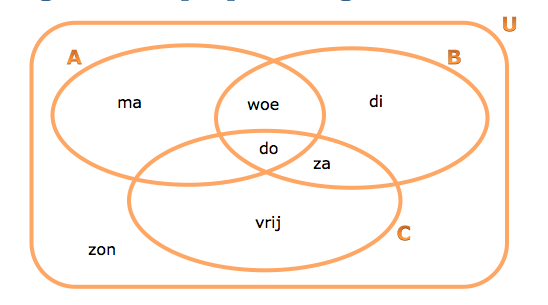
\includegraphics[width=0.7\textwidth]{figuren/verzamelingen_relaties/oefeningLeentje}
%
%\end{figure}
Zij $U$ de dagen van vorige week; $A$ de dagen met zon; $B$ de dagen met kou; $C$ de dagen met regen (figuur~\ref{fig:dagen}).
\begin{figure}[htbp]
\centering
% oefening venn
\begin{tikzpicture}[thick]
\draw (-4,-2.7) rectangle (4,3.5) node [above] {$U$};
\draw \firstellipse node at (35:3.7cm) {$B$};
\draw \secondellipse node at (145:3.7cm) {$A$};
\draw \thirdellipse node at (270:2.3cm) {$C$};
\node at (0,3) {zo};
\node at (1.8,1.3) {di};
\node at (0,1.5) {wo};
\node at (-1.8,1.3) {ma};
\node at (1,0) {za};
\node at (0,0.4) {do};
\node at (0,-1) {vr};
\end{tikzpicture}
\caption{Dagen van vorige week, figuur bij oefening~\ref{oef:oefLeentje}}
\label{fig:dagen}
\end{figure}
\begin{enumerate}
\item Geef door omschrijving:
\begin{enumerate}
\item $A\intersect B$
\item $(A\intersect C)-B$
\item $(A\union C)-B$
\item $A^c\intersect B^c$
\item $B^c\intersect C$
\end{enumerate}
\item Geef door opsomming:
\begin{enumerate}
\item $B-(A\intersect C)$
\item $C-(A\union B)$
\item $(A\union C)^c-B$
\item $(A-C)^c$
\end{enumerate}
\item Duid aan op het venndiagram:
\begin{enumerate}
\item $A^c-C$
\item $B^c -C$
\item $(A-C)^c$
\end{enumerate}
\end{enumerate}

\begin{opl}
\begin{enumerate}
  \item \begin{enumerate}
          \item $\{x| x \text{ is een dag met zon en kou} \}$
          \item $\{x| x \text{ is een dag met zon en regen maar zonder kou} \}$
          \item $\{x| x \text{ is een dag met zon of regen maar zonder kou} \}$
          \item $\{x| x \text{ is een dag zonder zon en zonder kou} \}$
          \item $\{x| x \text{ is een dag zonder kou en met regen} \}$
        \end{enumerate}
  \item \begin{enumerate}
          \item $\{\text{di},\text{wo},\text{za} \}$
          \item $\{\text{vr} \}$
          \item $\{ \text{zo}\}$
          \item $\{ \text{di},\text{do},\text{vr},\text{za},\text{zo}\}$
        \end{enumerate}
\end{enumerate}
\end{opl}
\end{oef}

%%% Local Variables: 
%%% mode: latex
%%% TeX-master: "../cursusTW1"
%%% End: 
